\chapter{Practical Aspects}
\label{chap:practical}

\myLettrine{G}{iven} the previously described topology and ideal model of the proposed solar inverter system in \chapref{chap:solution}, there is a need to implement this solution into a physical circuit in order to effectively determine the efficiency of this implementation.
This step is achieved by creating the design of a dedicated \gls{pcb} that contains the \gls{H-bridge}, passive filtering circuitry and logic control sections, combined with the \gls{pid} controller and current measurements implemented at the software level.
The solution I am proposing in the following sections have been made with these energy targets in mind:
\begin{itemize}
    \item Input voltage ($V_{in}$) is $24V$ \gls{dc};
    \item Output voltage ($V_{out}$) is $12V$ \gls{ac};
    \item RMS current converted ($I_{RMS}$) is around $2.5A$;
\end{itemize}
thus converting the equivalent of $30W$.
These characteristics are only ideal, as there are no perfect components and energy losses are unavoidable, however for the scope of this thesis, this should be enough to demonstrate the efficiency of the chosen topology.

\section{Hardware Implementation}
\label{sec:hwimp}

The process of designing the electronic device is split into choosing the main components (microcontroller, switching elements, current measuring resistor, operational and instrumentation amplifiers, passive components specific to the filtering), drawing the schematic of the board, simulating the design and doing the \gls{pcb} layout.
This has been done using KiCad, a free and open source CAD program that has more than enough features to aid in the development of the \gls{pcb} in question.

\subsection{Component Selection}
\label{subsec:compsel}

Arguably the most important section of the whole circuit is the \gls{H-bridge}, which allows for the formation of the current sine wave present in any \gls{ac} signal.
In most common instances, the bridge is composed of 4 transistors, either MOSFETs or IGBTs, that act as electronically commanded switches to the inverter system. On this prototype, size and cost are a priority over efficiency and maximum power rating, as long as these components can achieve the proposed target.
For this, I have chosen 2 IFX007Ts, which are \gls{ic}s containing a half-bridge and gate drivers, used primarily for motor control, but these can also be used in power conversion applications.
Since they can withstand up to $50A$ of current flowing through the drain and operate up to $40V$, these components satisfy the required targets.

Passive components chosen for the LCL filter are crucial in order to block residual high frequencies caused by the \gls{pwm} switching and any other external sources of noise\cite{reznik2013lcl, systematiclcl2015}.
Criteria for choosing these consist of low ESR values, which in turn would mean higher power conversion efficiency, tolerance values of the main characteristic of that component, maximum saturation current for the inductors and low ripple current for the capacitors.
Hybrid aluminum polymer capacitors exhibit such good values, and for inductors, specialized flexible transformer have been used, as the windings can be independently connected in serial and parallel configurations. This achieves different turn ratios, inductance and current-carrying capabilities.

\begin{figure}[!ht]
    \begin{center}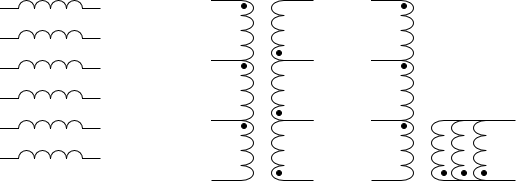
\includegraphics[width=\singlefigure]{\pics/schematics/transformerconfigs}\end{center}
    \caption{WE-FLEX transformer overview and example configurations}
    \label{fig:transf}
\end{figure}

The main take from \figref{fig:transf} is the following: the flexible transformer chosen can be thought of as 6 independent coils that can be connected in any way (as long as polarities are respected, market with a dot).
Knowing the base inductance per turn ($L_{base}$) is $12\mu H$ and the base current is $1.7A$, coils put in parallel multiply the base current rating, and windings put in series increase the inductance of the primary/secondary couple in accordance to this equation:
\begin{equation}
    \label{eq:Lwindings}
    L_{res}=L_{base} \cdot N_{sw}^2
\end{equation}
where $N_{sw}$ is the number of windings in series.
For the given examples, the middle configuration turns into a 1:1 ratio, $108\mu H$ transformer that can carry $1.7A$ of RMS current, and the right configuration is a 3:1 ratio transformer that has the same values on the primary as the former configuration, but the secondary can carry $5.1A$ with inductance $12\mu H$.

The feedback loop needs some way to have currents and voltages measured in order to calculate the next command to be given, thus a special current sense resistor is utilized in the circuitry.
This resistor has a low resistance value (usually under $1\Omega$), near 0\% tolerances and higher power ratings since they dissipate heat proportional to the current driven on the power traces, and it should not have its resistance drift with temperature changes.
Since we expect to deliver at least $2.5A$ RMS current through the \gls{pcb} traces, and to have minimal voltage drop across the resistor's terminals, I've chosen the WSLP2512R0100FEA, which is a $10m\Omega$, $\pm 1\%$ SMD resistor that can withstand $3W$ of power.
This is sufficient, as per Joule's first law:
\begin{equation}
    \label{eq:Joulefirstlaw}
    P = I^2 \cdot R
\end{equation}
it would result in a peak power dissipation of around $0.01\Omega \cdot (10A)^2 = 1W$, which is a third of the maximum power rating and a safe value to consistently maintain without damaging the component\cite{scherz2006practical}.

\begin{figure}[!ht]
    \begin{center}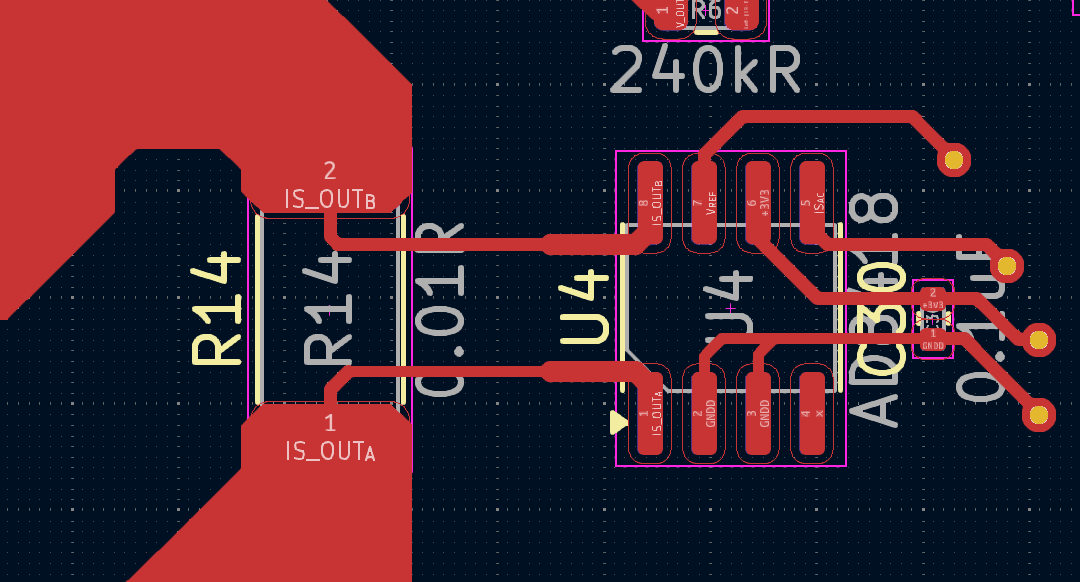
\includegraphics[width=\singlefigure]{\pics/schematics/kelvincon}\end{center}
    \caption{Example of Kelvin connections, voltage terminals come from inside the pads}
    \label{fig:kelvin}
\end{figure}

The voltage sensing terminals are then connected through \gls{Kelvin connection} (as shown in \figref{fig:kelvin}) to operational amplifiers and instrumentation amplifiers, like the MCP6001 and the AD8418 series respectively, used for amplifying the signal's gain and reject common-mode signals.
Current can't be directly measured, however the voltage drop on the shunt can be quantified, and since it is defined to be small in order to minimize losses, gain amplification needs to be done\cite{scherz2006practical}.
To calculate the source current, we can use Ohm's law:
\begin{equation}
    \label{eq:Ohmslaw}
    V = I \cdot R
\end{equation}
where the voltage is measured and resistance is already known.

All of these functions are tied to the microcontroller, that converts the values measured of the analog signals using the \gls{adc}s into numeric values, and these values are used as reference and system output in order to recalculate the \gls{pwm} duty cycles which modulates the carrier signal through the \gls{gpio}, or in this case, the converted \gls{ac} power source.
As discussed in \secref{sec:simrec} the period of the \gls{pwm} signal has been chosen to be of $20\mu s$, so any microcontroller which can output 50KHz signals and can calculate the next duty cycle in the meantime is fit for this project.
The choice of PSoC3M5 series has been mostly arbitrary, with the mention that ARM microcontrollers have been a popular choice in recent years as the CPU's architecture is easier to integrate into more complex SoCs.
Given the fact that it integrates 16 \gls{adc} channels, all digital pins have the capability of \gls{pwm} output, can operate at up to 180MHz and has numerous \gls{gpio} pins for additional expansion of functionality for debugging processes, it should be more than enough for this application.

\subsection{Electronic Circuit Overview}
\label{subsec:cirtdesc}

\begin{figure}[ht]
    \begin{center}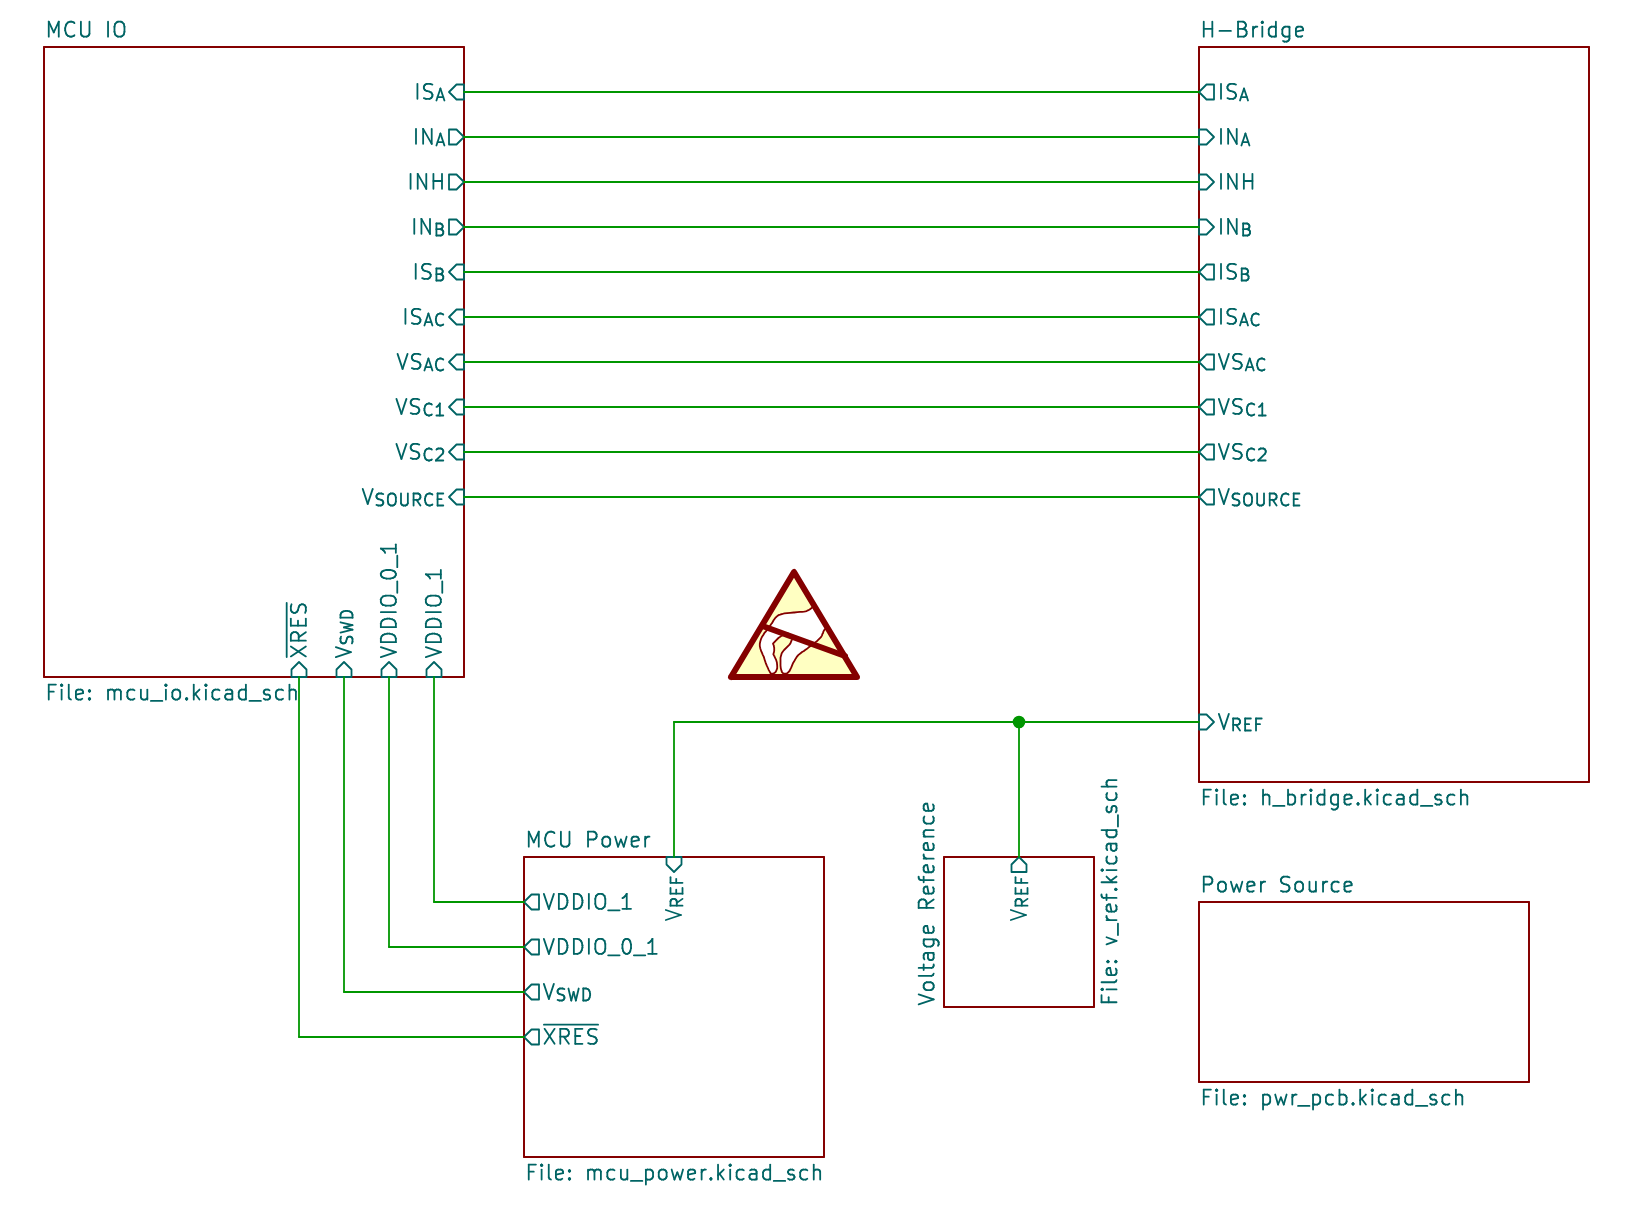
\includegraphics[width=10cm]{\pics/schematics/mainsch}\end{center}
    \caption{Schematic being split into functional blocks, with interconnects}
    \label{fig:mainsch}
\end{figure}

Once main component selection is done, the next step in designing the solution is to create the schematic of the circuit in order to describe how each of the parts will be connected together to form the power conversion topology, logic control and auxiliary power supply for the board to function.
It is important to note that in its description, the schematic representation is different from the layout, as the former shows at a functional level how each component is connected, while the latter contains the physical representation of these connections and other board properties such as layer definition and stack up and component placement.
To make the design easier to understand, the schematic has been split into multiple sections, as shown in \figref{fig:mainsch}.

The appropriately named \textit{H-Bridge} is responsible for the \gls{dc}-\gls{ac} conversion using the transistor bridge using 2 IFX007T as discussed in the previous subsection. The input current from the source, denoted by the connector $J1$ is passed to each half bridge \gls{ic}s, controlled using the signals $IN_{A}$, $IN_{B}$, and common inhibit signal $INH$.
$IN_{A}$ and $IN_{B}$ are the signals setting up bridge configuration; these should always have opposite values to prevent short-circuits.
$INH$ is the signal which modulated using \gls{pwm} would regulate the current conduction through its respective transformer connected to in series.
The output of each \gls{ic} is then passed through the LCL filter, which utilizes the transformers in 2 stages: the first has all of the windings connected in parallel ($T1$ and $T2$), which would form a $12\mu H$ inductor, while the second transformer ($T3$) is configured as a series of 3 groups of 2 parallel windings that results a $108\mu H$ value.

\begin{figure}[!ht]
    \begin{center}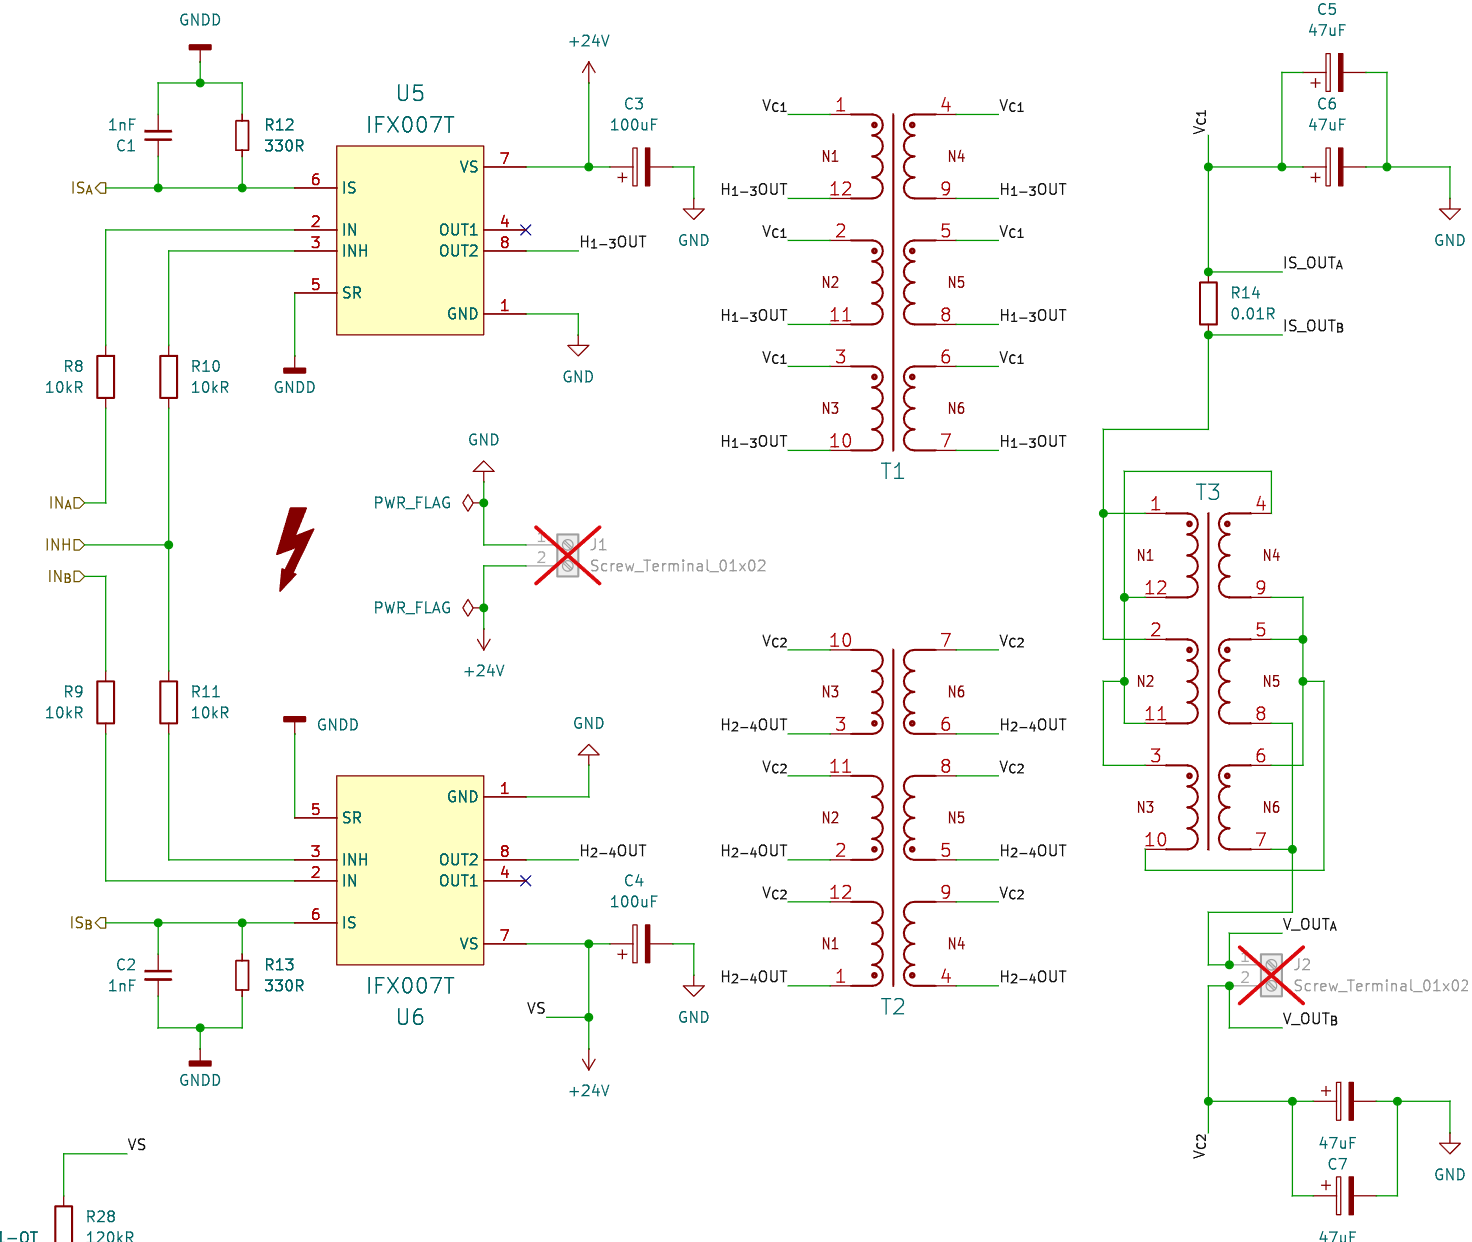
\includegraphics[width=\singlelongfigure]{\pics/schematics/hbridge}\end{center}
    \caption{Schematic of the implemented topology}
    \label{fig:hbridgesch}
\end{figure}

While the expected voltage that is injected into the grid through $J2$ should be 24V, to be sure that the feedback loop is correctly implemented, dedicated measurement circuitry is added on the board to know output voltage, output current that the board regulates through the $R12$ shunt, input source voltage (denoted through the $VS$ label), and voltages across both arms of the low-pass filter.

\begin{figure}[!ht]
    \begin{center}
        \subfloat[output voltage]{\label{fig:getvout}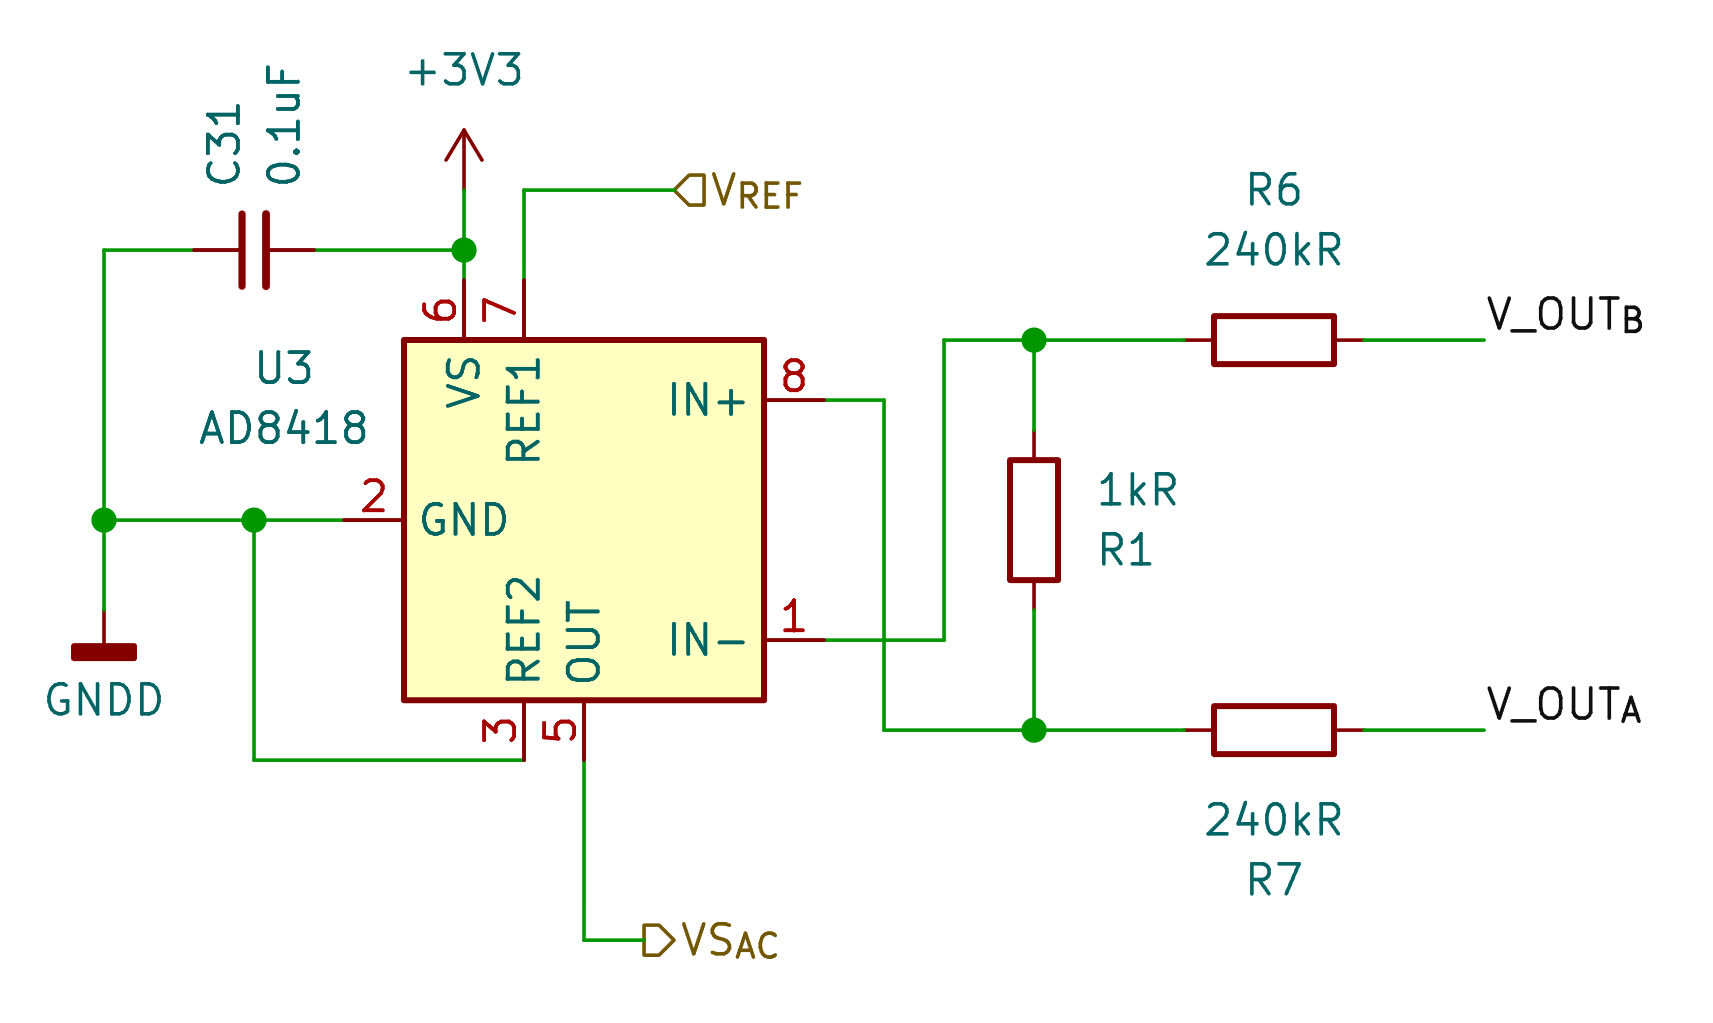
\includegraphics[width=\triplefigure]{\pics/schematics/voltageshunt}}
        \subfloat[output current]{\label{fig:getiout}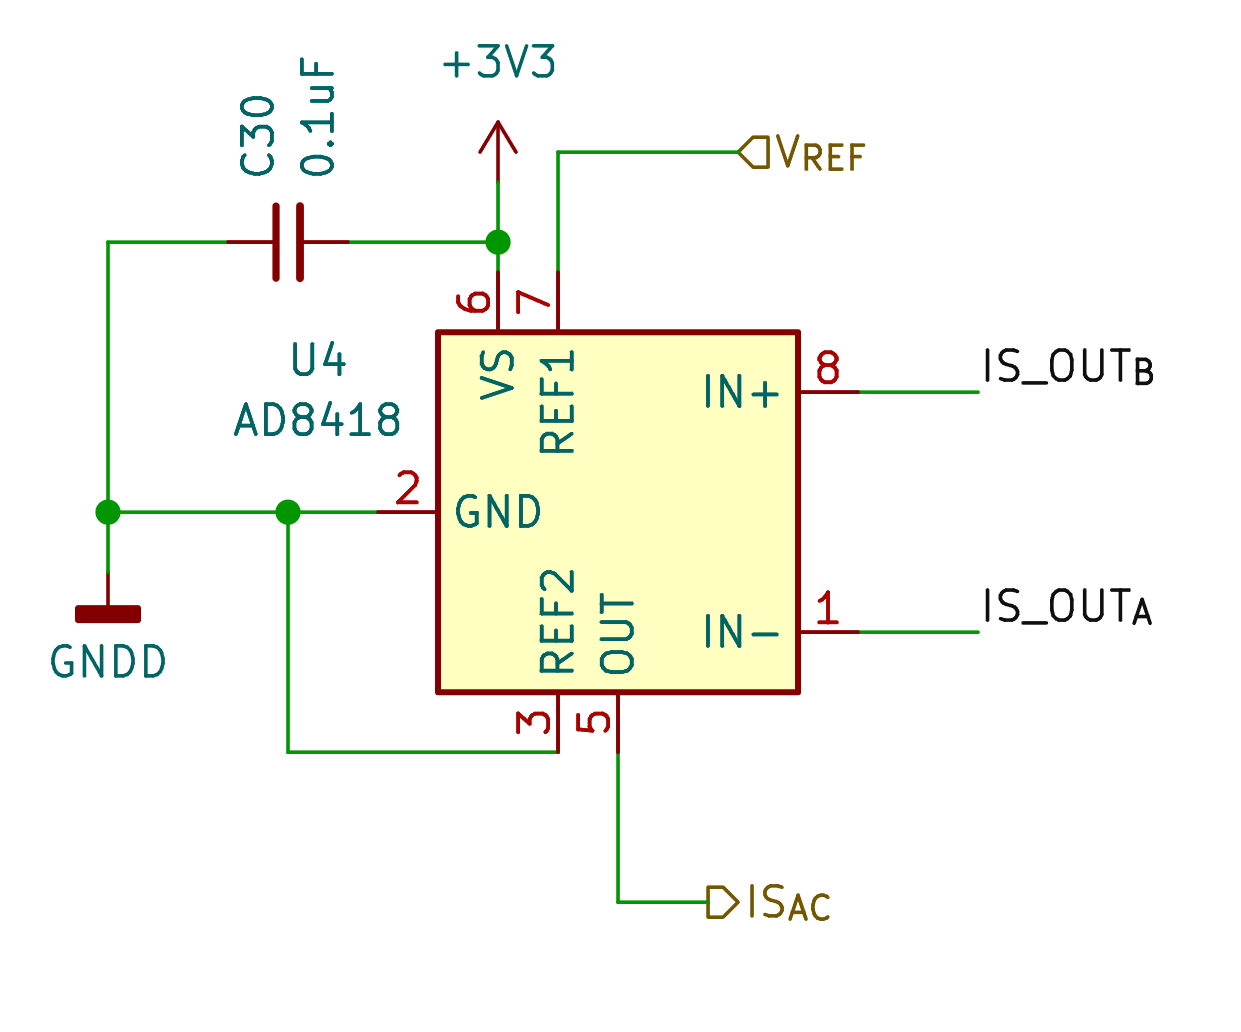
\includegraphics[width=\triplefigure]{\pics/schematics/currentshunt}}
        \subfloat[input voltage]{\label{fig:getvin}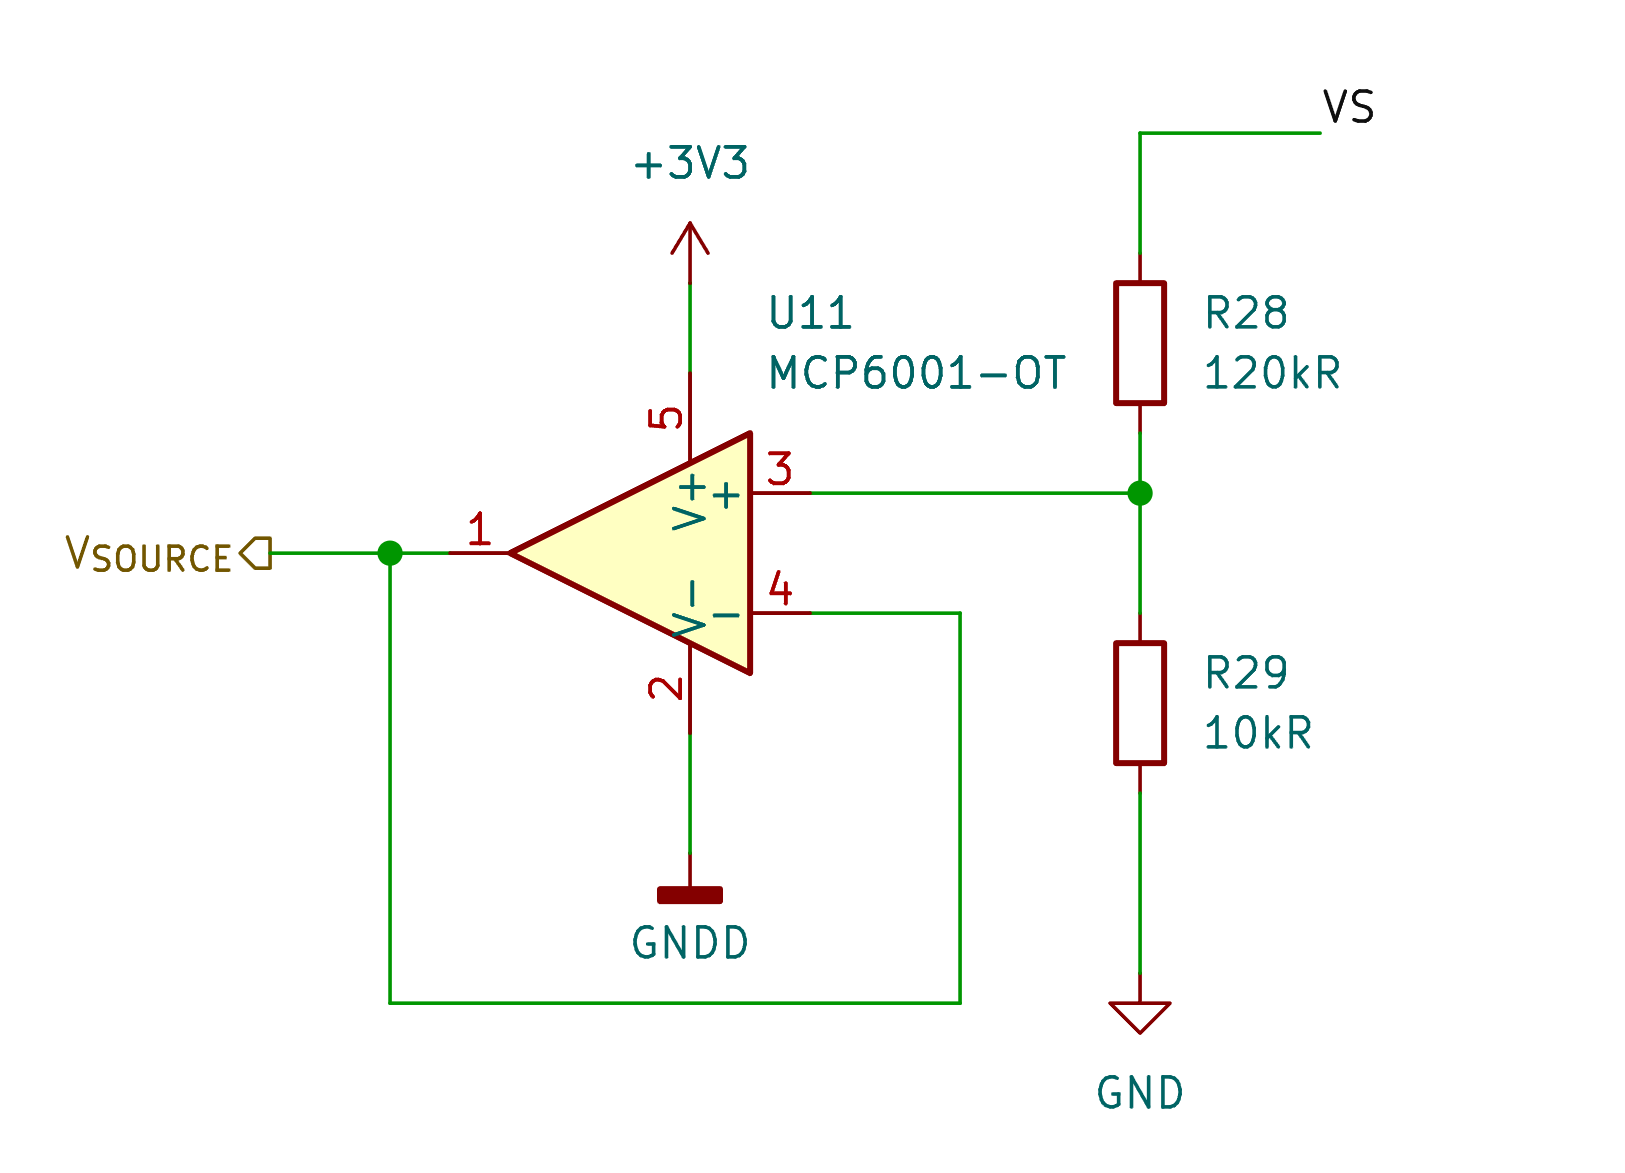
\includegraphics[width=\triplefigure]{\pics/schematics/opamp}}
        \caption{Amplifiers used in voltage and current measurements}
        \label{fig:omapms}
    \end{center}
\end{figure}

For both output voltage and current, I have applied a differential measurement method as to isolate the common-mode noise that may arise in supply switching circuits, as this can negatively impact the readings on the \gls{adc}.
In \figref{fig:getiout} the load is measured at the connections points under the resistor pads, with minimal voltage dropout as the resistance is significantly small ($10\mu \Omega$).
On the output voltage, the resistor network used in \figref{fig:getvout} is used to match the impedance across both segments, and $R1$ is used to adjust the gain of each input of the instrumentation amplifier.
For the input voltage (\figref{fig:getvin}), a sensing wire is connected at the positive terminal of the source terminal, and the value is reduced to $\approx 7.69\%$ using the voltage divider.
This same circuit is also used to measure the voltage across each arm of the bridge, in order to know the voltage at the capacitors, for nets $V_{C1}$ respectively $V_{C2}$.
Finally, each half bridge \gls{ic} contains a current sense signal $IS$ that can be utilized to either report the current flowing through the \gls{ic}, or to alert of overcurrent events.

\begin{figure}[!ht]
    \begin{center}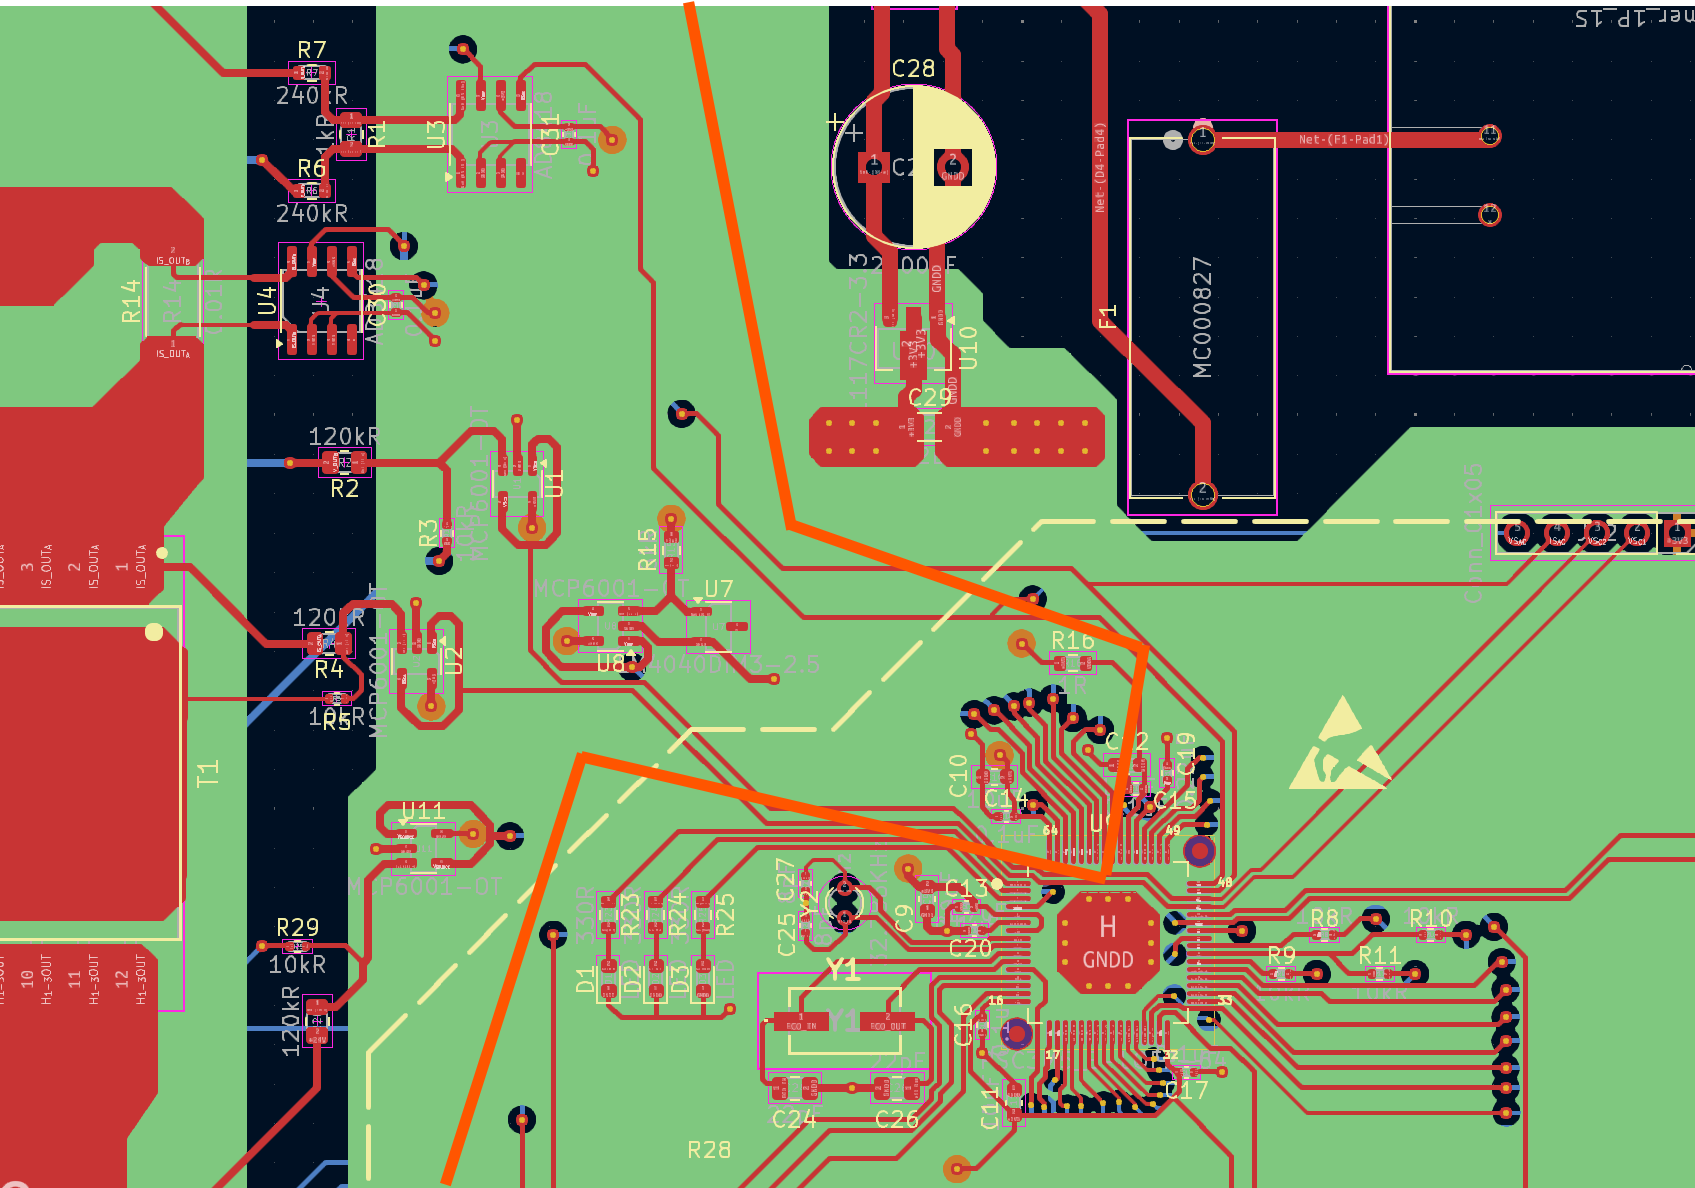
\includegraphics[width=\singlefigure]{\pics/schematics/analogzone}\end{center}
    \caption{Split by the orange line, analog signals are separated from digital wires}
    \label{fig:analogzone}
\end{figure}

Control and measurement signals used in the feedback loop have the direction of flow represented in \figref{fig:mainsch}, going to and from the \textit{MCU IO} block.
The separation in schematic is not only physical, as the number of peripherals connected to the microcontroller require space in order to be properly laid out.
These signals should be routed to accommodate for the electrical requirements in order to avoid induced noises and significant voltage drops.
Mainly, voltage and current measured are analog signals and have to pass through the \gls{adc}s, meaning that the wires should be physically as far as possible (depicted in \figref{fig:analogzone}) from any digital signals, and especially switching pulses, like the $INH$ signal\cite{zumbahlen2007basic}.
Besides control signals, other auxiliary ports are connected to the microcontroller to allow the users to implement additional functionalities depending on the application, but most importantly to create mechanisms for emergency stops or to point out the functioning state of the hardware and to upload and debug the program to be written on the microcontroller.

\begin{figure}[!ht]
    \begin{center}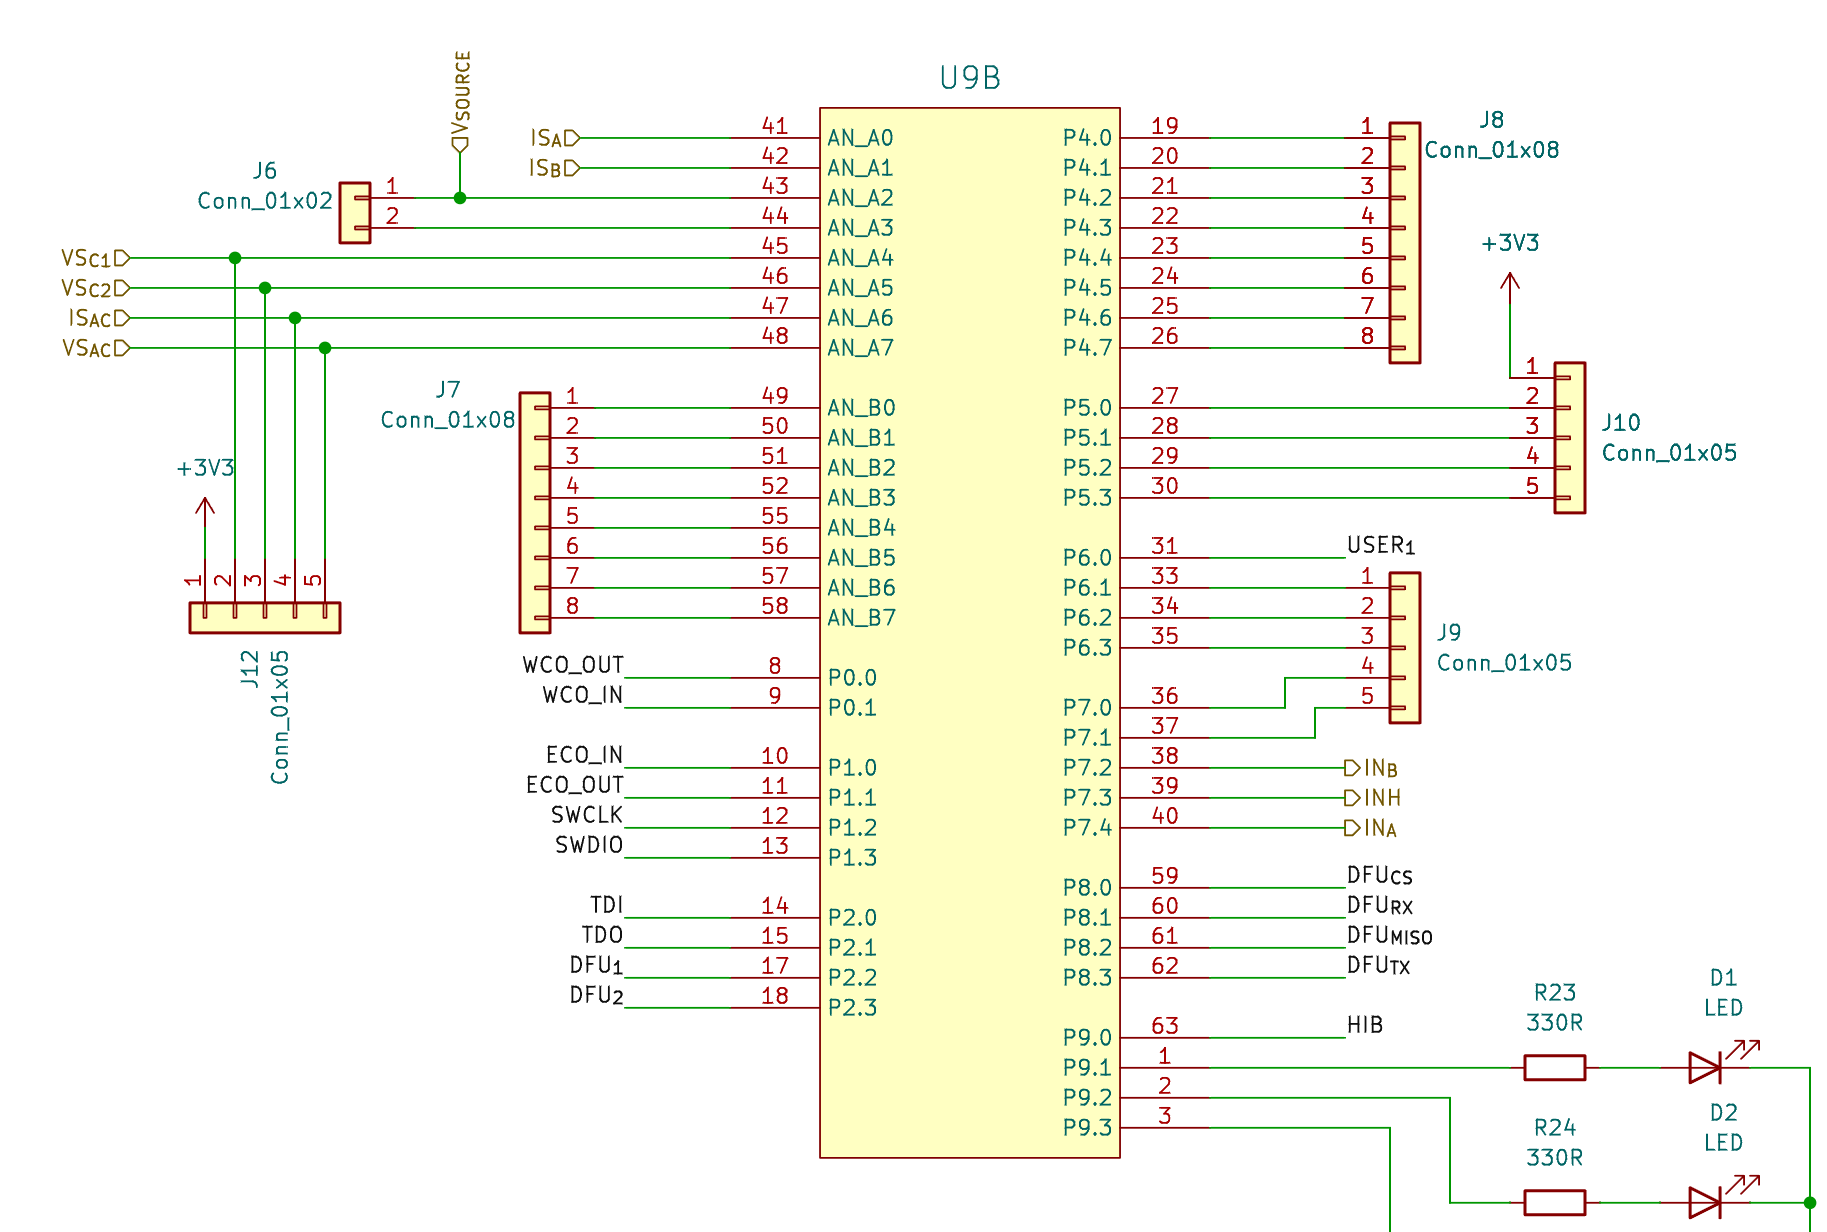
\includegraphics[width=\singlelongfigure]{\pics/schematics/mcuio}\end{center}
    \caption{Schematic representation of the I/O connections}
    \label{fig:mcuio}
\end{figure}

Even if the board already has a power input coming from the supposed photovoltaic cell, the energy provided is unreliable to supply critical areas responsible for converting the power, and besides that, another stage of voltage step-down has to be implemented in order to deliver the low voltages at which the logic circuits function at [$3.3V, 5V$].
Instead, the board has to be powered on by an individual power supply, which could give some flexibility in how the solution can draw supply rails to each \gls{ic} and can reduce the footprint on board.
There cold be multiple ways to create this architecture, but in the end, I have chosen to include a classic step-down transformer with a diode rectifier in order to power the circuit from any \gls{ac} source.
This option would ease the development of the board as energy coming from the grid is already subjected to strict control, thus requiring less components to filter the resulting input current.
For powering the components, there are 2 solutions to draw the supply rails: either have separate wires for each power domain, and in this case, separation from discrete and analogic devices, or spread the components' placement across a dedicated power plane\cite{zumbahlen2007basic}.
Since circuit requirements are not stringent, as long as current paths do not cross from one domain to another, a dedicated power plane may be sufficient for proper operation.

This leads to the final consideration of the board, deciding the stack-up of the \gls{pcb}.
Considering the previous discussion about component layout and power supplying solutions, I have decided to use a 4-layer board, each with their own signal category assignment.
\figref{fig:stack} contains a sliced representation of the board showing each layer and their attribution, matched to the color of the layer as presented in KiCad.

\begin{figure}[!ht]
    \begin{center}
        \subfloat[H-bridge section]{\label{fig:stack1}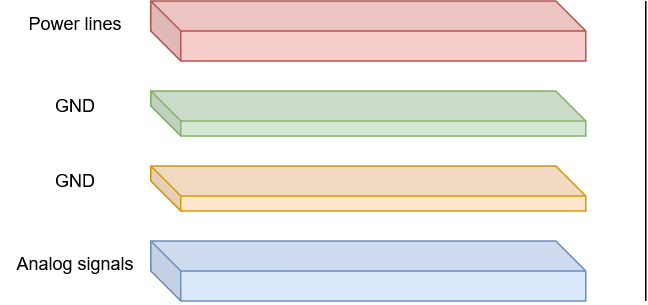
\includegraphics[width=\doublefigure]{\pics/schematics/layers2}}
        \subfloat[Logic control section]{\label{fig:stack2}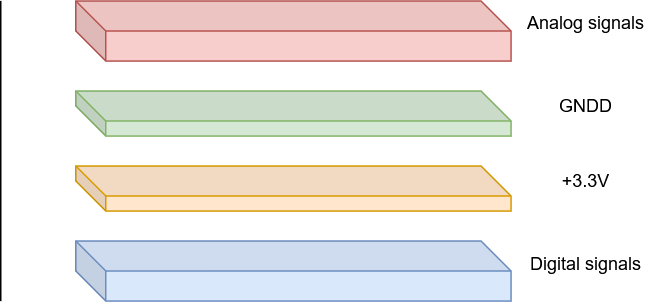
\includegraphics[width=\doublefigure]{\pics/schematics/layers1}}
        \caption{PCB stack-up}
        \label{fig:stack}
    \end{center}
\end{figure}

For \figref{fig:stack2}, the chosen order is standard in 4-layer board, made in such a way to minimize the interferences between mixed domain signals, and to decouple the analogic section from the power plane by shielding it with the ground plane.
On the power conversion section, the most important requirement is to design the traces in such a way that the board does not overheat and cause malfunction.
As suggested in both sections, outer layers have a larger cross-section than the inner layers, thus are more suitable for conducting high currents through them.
For improved thermal dissipation, maximizing the width of any trace can lead to further heat spread, and where possible, instead of using traces, copper pools can be utilized to accomplish this technique, as shown in \figref{fig:gerberbridge}.
Inner layers on this section only have shielding effect in order to reduce \gls{emi} spreading to the voltage sensing lines.

\begin{figure}[!ht]
    \begin{center}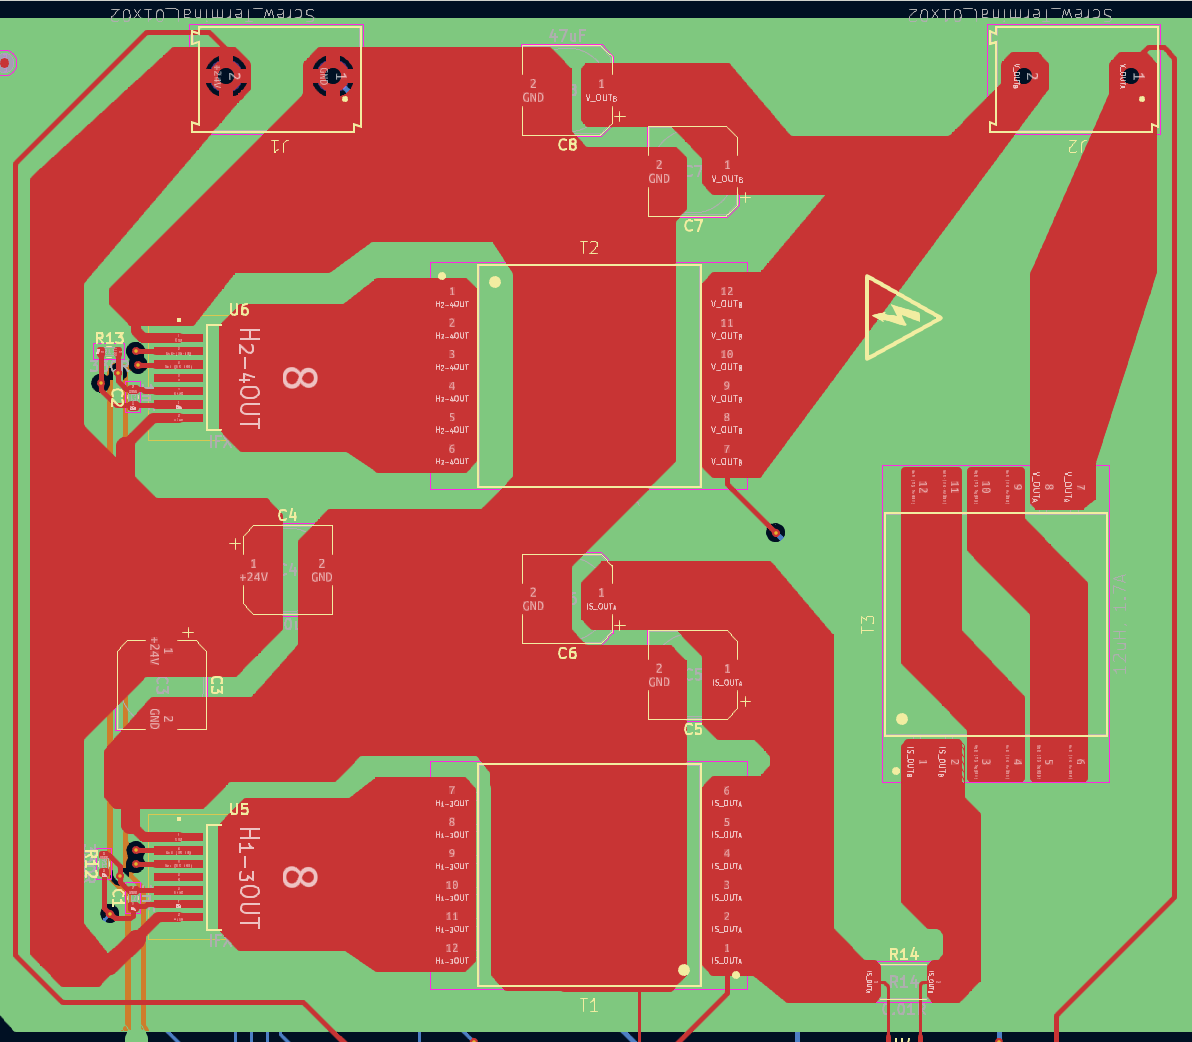
\includegraphics[width=\singlefigure]{\pics/schematics/gerberBridge}\end{center}
    \caption{Copper fill areas in red show the high voltage traces as spread out}
    \label{fig:gerberbridge}
\end{figure}

\section{Software Implementation}
\label{sec:swimp}

As expected from the previously described design, the active circuits present on the board have to be driven by the control algorithm in order for the system to properly function.
The most important component that orchestrates this aspect is the microcontroller, that hosts the peripherals necessary in order to measure both the system's parameters and to compute the \gls{pwm} duty cycle.
When talking about the software's architecture, besides the CPU that is responsible for scheduling the program and to calculate the next time period, there is a need to mention the dedicated hardware peripherals inside the microcontroller that facilitate physical to digital connections which make the solution function.
In \figref{fig:swarch} is presented how the peripherals are logically connected in order to create the control algorithm.
\begin{figure}[!ht]
    \begin{center}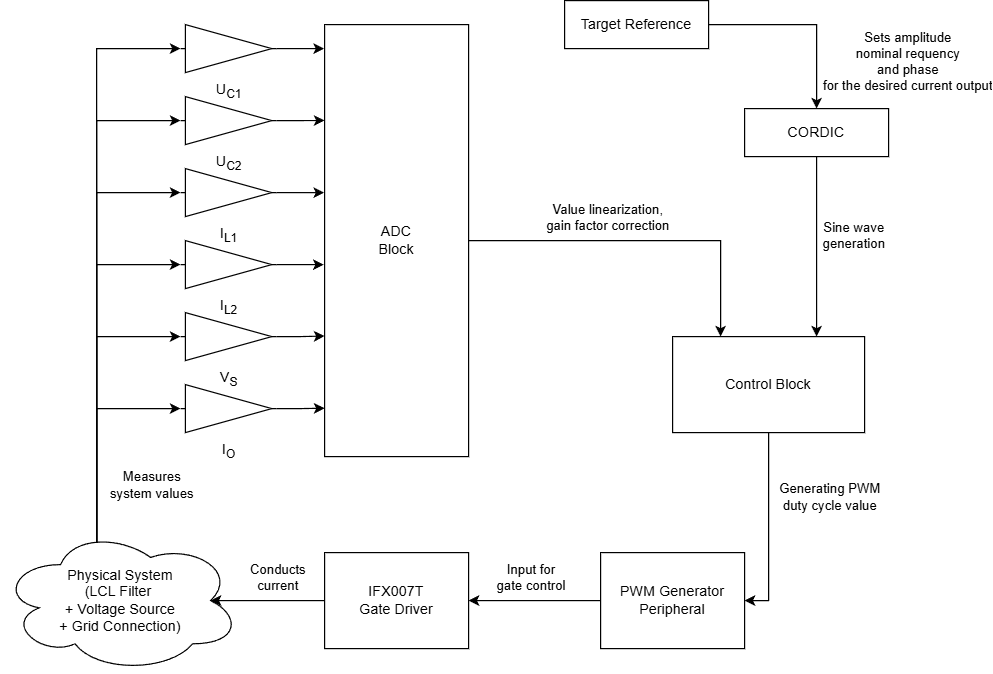
\includegraphics[width=\singlefigure]{\pics/schematics/swarch}\end{center}
    \caption{Logical representation of software architecture and peripheral usage}
    \label{fig:swarch}
\end{figure}

In layman terms, the physical circuit works in the continuous domain, meaning each current and voltage is corresponding to the analog domain.
It is not enough to only measure these, but to convert them using the \gls{adc} peripheral, which would give raw numeric values.
This block can also scale these values to floating point voltages and currents based on the PSoC3M5's documentation that implements a function call.
For the control algorithm, we need to have the output inductor's current, grid voltage, source voltage and at least one of the capacitor's voltage, since in theory, the capacitors have a complementary voltage that averages to the output source voltage.
Since the \gls{adc} peripheral can work up to 240MHz, and it takes a minimum of 4 cycles for the results, the average response time for the conversion is around $16.66\mu s$ \cite{psocdatasheet}.
If the \gls{pwm} sampling frequency is chosen as 50KHz, the \gls{pwm} counter has 1200 values, or an 11-bit resolution, which is sufficient for precise commands.
As the \gls{adc} block functions independent of the CPU, there is no need to optimize the scheduler to take each conversion into account, as once the operation is done, we can trigger the peripheral to update the measured values to the software.
The same procedure is done for computing the reference value for the desired sine wave, as we can offload the workload from the CPU to the CORDIC block.
CORDIC is a special hardware acceleration block that can compute trigonometrical functions and the square roots much faster than traditional software methods, meaning it is appropriate in this instance to update the reference sine wave every \gls{pwm} time period.
Having all of the necessary values to compute the next duty cycle, the CPU them computes the correct command that is sent to the \gls{pwm} signal generation block.
To drive the MOSFETs inside the IFX007T, there are 3 signals used as follows:
\begin{itemize}
    \item ${INH}$ is the signal driven using \gls{pwm}, that is common to both half-bridges;
    \item $IN_A$ and $IN_B$ are driven complementary; when one half-bridge drives the high-side transistor, the other should also open the low-side transistor for allowing the system to function under \gls{dcm}.
\end{itemize}